%************************************************
\chapter{Data Analysis at the LHC}\label{ch:introduction}
%************************************************
The LHC produces -at design parameters- over 600 millions collisions ($\approx 10^9$ collisions) proton-proton per second in ATLAS or CMS detectors. The amount of data collected for each event is around 1 MB (1 Megabyte). This means that we are reaching 1 PB/s (1 \emph{Peta}byte/second) of data--far too much for any detector data acquisition system to handle.

The trigger systems alleviate the problem by reducing the amount of data by a factor of 1000 or 10000; despite this, the constant need of cutting-edge resources and solutions, both in hardware and software, have been driving extremely fruitful research in the history of the LHC.

One major necessity, whose importance and scale may not be appreciated by people outside of the field, is the one for \emph{simulations}.

\section{The necessity of simulations}

First of all, why do we need simulations in the first place?
The simulation is a crucial aspect of any high energy physics experiments. In CMS it is used both
at analysis level and for testing the algorithms before deployment with data. The simulation targets relatively rare processes originating from a hard interaction between two
proton components, which are signal or background for specific analyses. Single particles
or hadronic jets can also be simulated for specific purposes.

Simulations are a necessity if we have to test a physical theory: we need to know what reality would look like if the proposed theory was true or not. Then we can check which hypothesis our data looks like, and we can either validate or disprove the theory.

Without a proper simulation, we also would not know the expected performance of the detector and the regions of interest for our process, making it impossible to correctly operate the apparatus and obtain reasonable results.

\section{Modelling an event}

There are three major, distinct steps in modelling a physical event at CMS. The first one is more generally related to the physical theories and calculations, while the other two are specific to the CMS detector. The whole process is often referred to as \emph{FullSim} (full simulation).

\subsection{Event generation}

The first step to any good simulation is called \emph{generation}, that is all the calculations based on Quantum Chromodynamics which describes how the quarks and gluons inside the protons scatter off one another, how they might create new particles, and how those new particles behave after they have been created. 

Proton-proton collisions are very complex and difficult to model accurately. Protons are
composed of 3 quarks, called \emph{valence} quarks, by virtual gluons and virtual quark anti-quark
pairs coming from gluon splitting. All constituents of hadrons are generically called \emph{partons}.
During high energy collisions, the protons behave as a collection of free partons and the
hard scattering can be described at the level of parton interactions. The hadronic cross
section $\sigma_{pp}$ is calculated based on the QCD \emph{factorization} theorem. The factorization theorem
states that the hadronic cross-section $\sigma_{pp}$ is a convolution of the partonic cross section  $\hat{\sigma}_{ij}$ with the parton distribution functions (PDFs) $f_i(x)$:

\[
\sigma_{pp} = \int_{x_{min}}^1 dx_1 dx_2 \sum_{i,j}f_i(x_1)f_j(x_2)\hat{\sigma}_{ij}(x_1 p_1, x_2 p_2)
\]

where function $f_i(x)$ is probability density that a parton of type i has a fraction x of the
hadron energy. The final cross section may be evaluated by the single, non-trivial contributions $\hat{\sigma}_{ij}$.

Apart from the hard interaction, the other constituents of the proton can also interact. This
usually results in a spray of softer particles, called \emph{underlying event} (UE). Any high momentum particle involved in the collision will emit additional hard QCD radiation. Radiation
from particles before the hard interaction is called \emph{initial-state-radiation} (ISR), whereas radiation off particles produced in the collision is called \emph{final-state-radiation} (FSR). Quarks and gluons can emit additional radiation via the strong interaction. All the quarks
and gluons go through the hadronization process, forming colorless hadrons. Finally, unstable particles are going to decay. A representation of all these elements is shown in Figure \ref{fig:evgen}.          

\begin{figure}
    \centering
     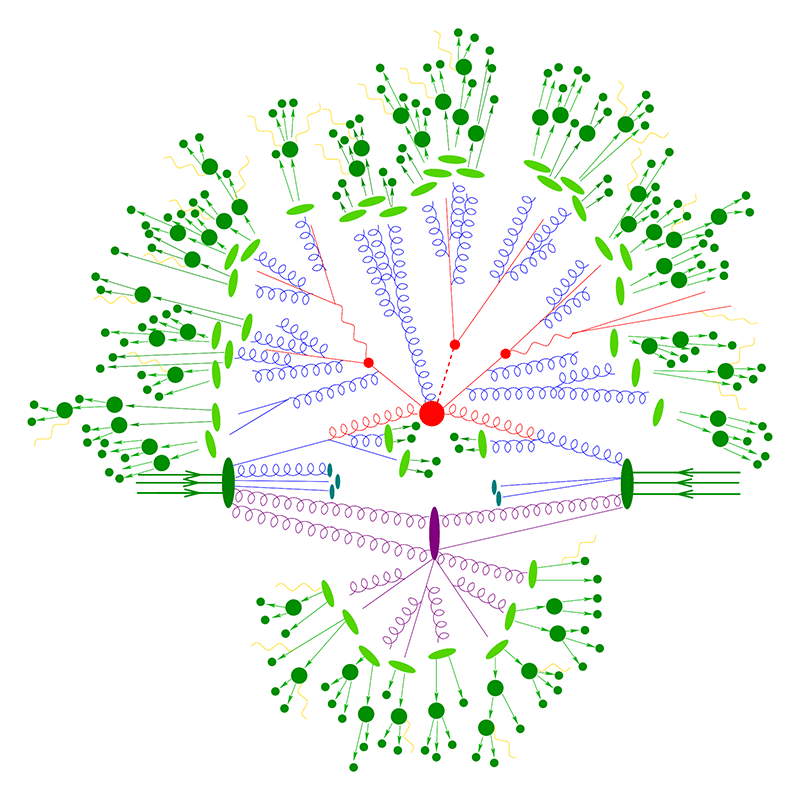
\includegraphics[width=.65\linewidth]{gfx/ch2/event_800px.png}
    \caption[Event generation]{ Representation of a proton-proton collision event. The red part includes the hard interaction and the decay of the products. Initial and final state radiation are in blue. A secondary
interaction can take place, in purple, before the final-state partons hadronize. The hadronization is
represented by the green blobs, and the hadron decay in dark green. Photon radiation is in yellow. From \cite{evgen}.}
    \label{fig:evgen}
\end{figure}


All the various parts involved in this step can be summarized as:

\begin{outline}
    \1  The PDFs that are phenomenological functions computed using experimental information;
    \1  the hard scattering, computed perturbatively order by order;
    \1  the parton \emph{showering}, used to simulate additional emissions in perturbative QCD;
    \1   the hadronization, describing the transition from colored particles to hadrons, treated
        using phenomenological models;
    \1   the decay of unstable particles, modeled based on experimental data.
    
\end{outline}

The first two are usually included in \emph{Matrix Elements generators}, while the last three are
included in Parton Showering programs. Both use Monte Carlo techniques; some popular multi-purpose generators include \texttt{Pythia8}, \texttt{MadGraph} and \texttt{Sherpa}.

We can thus obtain a complete description of all the (stable) particles that come out of a collision between two protons under our theory only after a complex process involving several months of modelling and calculations.

\subsection{Detector Simulation through GEANT4}

Now that we have the particles resulting from our process, we must take the detector into account. This means simulating all the interaction processes that are going to happen between particles and matter by moving them through the detector one by one and modelling the detector’s response to each one of the particles as it goes. 
Undoubtedly, the de-facto standard for such a task is the \texttt{Geant4} toolkit (see \cite{AGOSTINELLI2003250}). It is intended to simulate the passage of particles through matter and it includes a complete range of functionality including tracking, geometry, physics models and hits. The physics processes offered cover a comprehensive range, including electromagnetic, hadronic and optical processes, a large set of long-lived particles, materials and elements, over a wide energy range starting, in some cases, from 250 eV and extending in others to the TeV energy range. It has been designed and constructed to expose the physics models utilised, to handle complex geometries, and to enable its easy adaptation for optimal use in different sets of applications. The toolkit is the result of a worldwide collaboration of physicists and software engineers, created exploiting software engineering and object-oriented technology and implemented in the \texttt{C++} programming language.

\begin{figure}
    \centering
     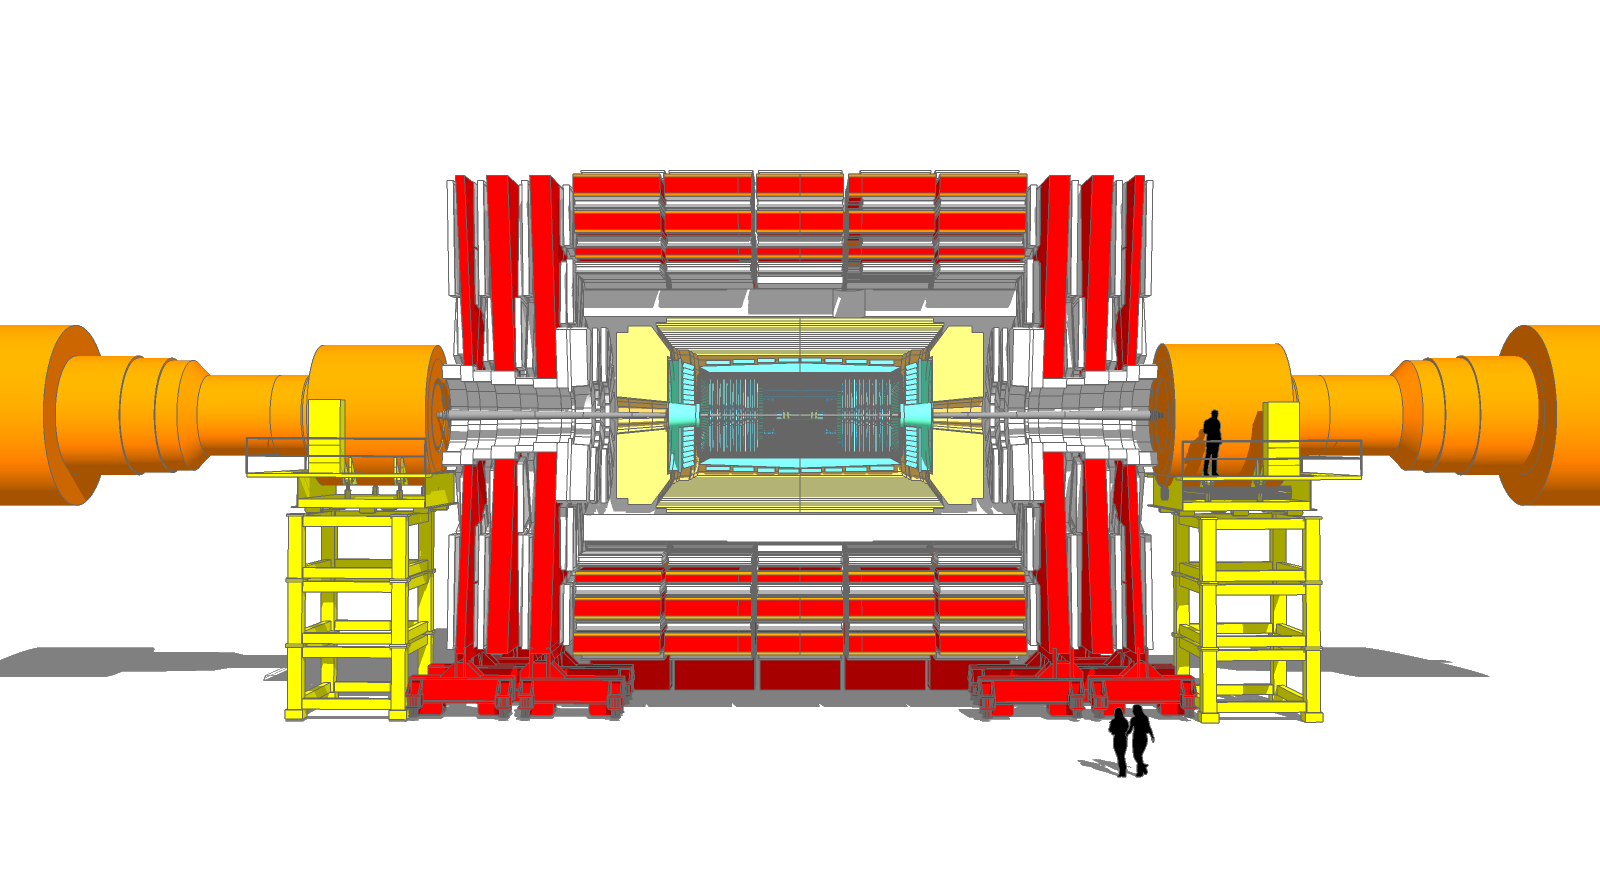
\includegraphics[width=\columnwidth]{gfx/ch2/cms_160518_01_Scene_2.png}
    \caption[CMS model]{ Representation of the CMS detector based on the actual \texttt{Geant4} CMS Detector Description. It accurately and precisely reproduces the geometry of all CMS detector subsystems, including the geometries of the original CMS detector, phase 1 and phase 2 upgrades.  From \cite{decmod}}
    \label{fig:decmod}
\end{figure}


However, \texttt{Geant4} can only provide us with a description of the single physical processes and materials, so we need to provide the actual \emph{detector description} (see Figure \ref{fig:decmod}). 

Every piece of the detector has to be put together, with the right material assigned to each. The full detector description has millions of volumes and hundreds of different materials. There is a selected group in CMS realizing technical drawings (and photographs, as the technical drawings are not always accurate) of the detector and translating them into something \texttt{Geant4} can use. As the simulation would be far too expensive if we considered all of the actual components, at time it is necessary to define specific \emph{shortcuts} which do not impare the reliability of the simulation too much. It’s a painstaking process, still ongoing today as a continuous refinement and improvement of the current model.

Next comes the set of physics models. The toolkit has a great variety of them that you can use and they have a default quite suited to the HEP use case. Those physics models describe each process (e.g. the photoelectric effect, Compton scattering, bremsstrahlung, ionization, multiple scattering, decays, nuclear interactions, $\dots$) for each particle. Some calculations can be very complicated and costly, so we have to choose, at this point, what physics we aree interested in. \texttt{Geant4} can be used for simulation of space, simulation of cells and DNA, and simulations of radioactive environments. It is usual to take the fastest model whose results we cannot really distinguish from the most detailed models. That is, we turn off everything that we don’t really notice in our detector anyway.

The last part is to specify the \emph{saving} options. \texttt{Geant4} does not inherently know the difference between some silicon that is a part of a computer chip somewhere in the detector and the silicon that makes up the sensors in the inner detector. So we specify the parts of the detector that are the most crucial, called \emph{sensitive} detectors. There are a lot of technicalities to optimizing the storage, but in the end we want to write files with all the energy deposits that  \texttt{Geant4} has made, their time and location – and sometimes information (called \emph{truth}) about what really happened in the simulation, so later we can find out how good our reconstruction software was at correctly identifying photons and their conversions into electron-positron pairs, for example.

At the end of this costly step, we are left with a long list of energy deposits, times, and locations in our detector. 

\subsection{Digitization and Reconstruction} 

The last part of the simulation process consists in turning the energy deposits into the actual signal outputted by the detector-- a process called \emph{digitization}, once again specific for the CMS detector.

The simple idea is to change the energies into the detector outputs – usually times, voltages, and currents, for example. We have to build in all the detector effects that we care about. Some are well known such as Birks’ law, for example; others are more complicated, like the change in light collected from a scintillator tile in the calorimeter depending on whether the energy is deposited right in the middle or on the edge. We can use the digitization to model some of the very low-energy physics that we don’t want to have to simulate in detail with \texttt{Geant4} but want to approximate to an average. Those are effects like the spread and collection of charge in a silicon module or the drift of ionized gas towards a wire at low voltage.

Digitization is where some other effects are put in, like the pile-up, the extra proton-proton collisions in a single bunch crossing. Those are usually pre-simulated and add on top of the important signal events. We can add other background effects if we want to, like cosmic rays crossing the detector, or proton collisions with remnant gas particles floating around in the beampipe, or muons running down parallel to the beamline from protons that hit collimators upstream. 

Finally, we also have to pass our simulated data to the track reconstruction and particle flow algorithms to obtain a collection of physical objects as reconstructed by the detector readout. This is the \emph{reconstruction} step, resulting in events similar to the one shown in Figure \ref{fig:cmsev} . Detector hits after the simulation and reconstruction steps are called \emph{SimHits}
and \emph{RecHits} respectively.

\begin{figure}
    \centering
     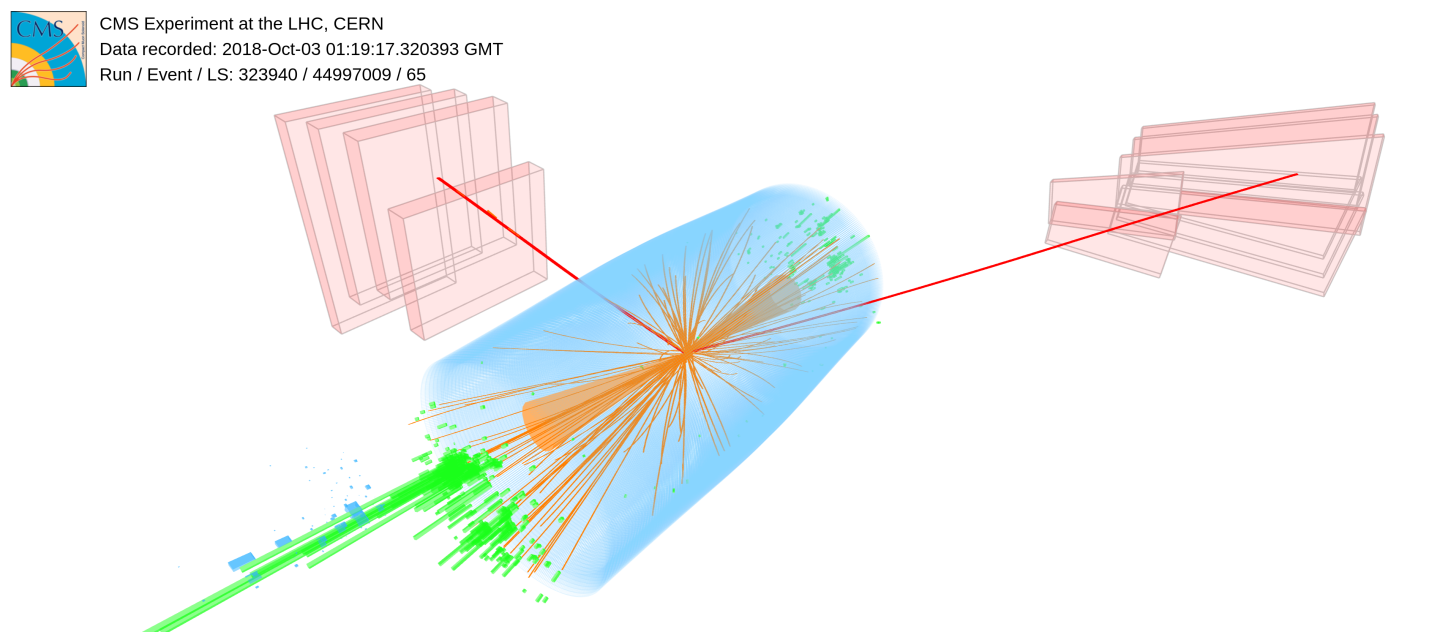
\includegraphics[width=\columnwidth]{gfx/ch2/HIG-19-006_VBF_white.png}
    \caption[CMS Event]{Event in which a candidate Higgs boson produced by vector boson fusion (VBF) decays into two muons, with an invariant mass of 125.01 GeV and per-event mass uncertainty of 1.83 GeV. The forward jets from the VBF are depicted by the orange cones and the muons are drawn as long red lines. Courtesy of the CMS Collection.}
    \label{fig:cmsev}
\end{figure}


At the end of the process we have something that looks exactly like the real data – except we know exactly what it is, without any ambiguity. With that, we can build up some simulated data that includes all the different processes that we already know exist in nature, like the production of top quarks, W bosons, Z bosons, and the Higgs bosons. And we can build another set that has all of those, but also includes other alternative theories. The last part, which is really what much of the data analysis is concerned with, is trying to figure out what makes events under the new hypothesis different from the other ones we expect to see – and trying to isolate them from the others. We can look at the reconstructed energy in the event, the number of particles we find, any oddities like heavy particles decaying away from the collision point – anything that helps. And we have to know a relevant information about the simulation, so that we don’t end up using properties of the events that are very hard to simulate to separate new particles from known ones. This is usually the first part of almost all the data analyses at the LHC, while the last one is the \emph{unblinding}, where we eventually check the data that has all the features we request – passes all our requirements – and see whether it looks more like the null or alternate hypothesis. Sometimes it can be useful to use \emph{data-driven} methods to estimate the backgrounds (or tweak the estimates from our simulation), but almost every time it is common to start from the simulation itself.

\subsection{Computing Costs}

Due to the length and the complexity of the process, its tremendous computation costs should not come as a surprise. Figure \ref{fig:cpuusage} shows the public approved HL-LHC CMS projections for the CPU usage at CMS.

\begin{figure}
    \myfloatalign
    \subfloat[]
    {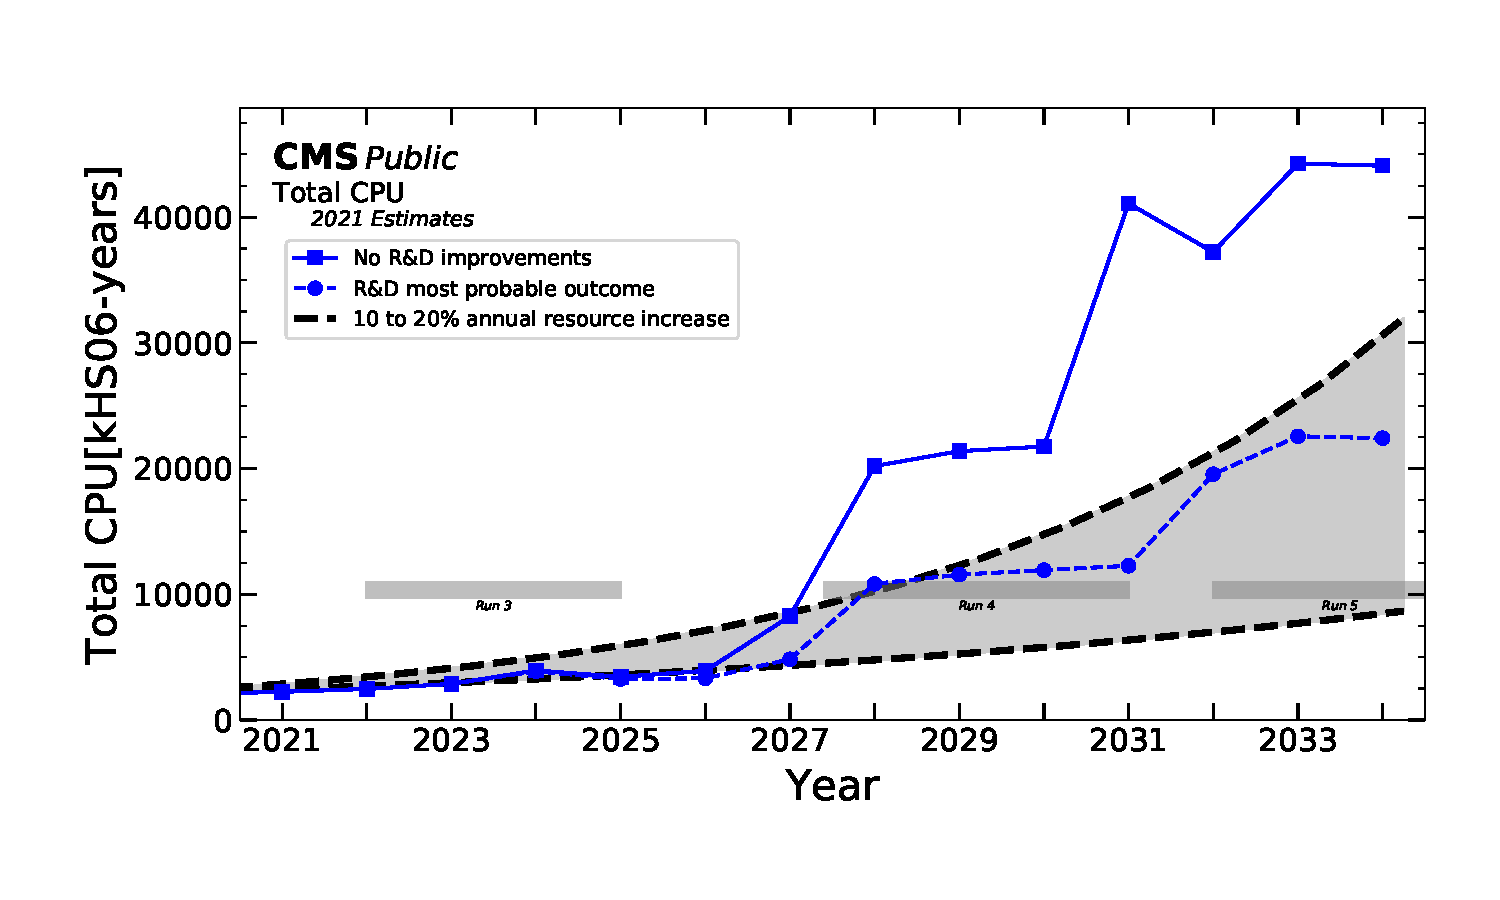
\includegraphics[width=.65\columnwidth]{gfx/ch2/cpu_cms2021.pdf}} \\
    \subfloat[]
    { 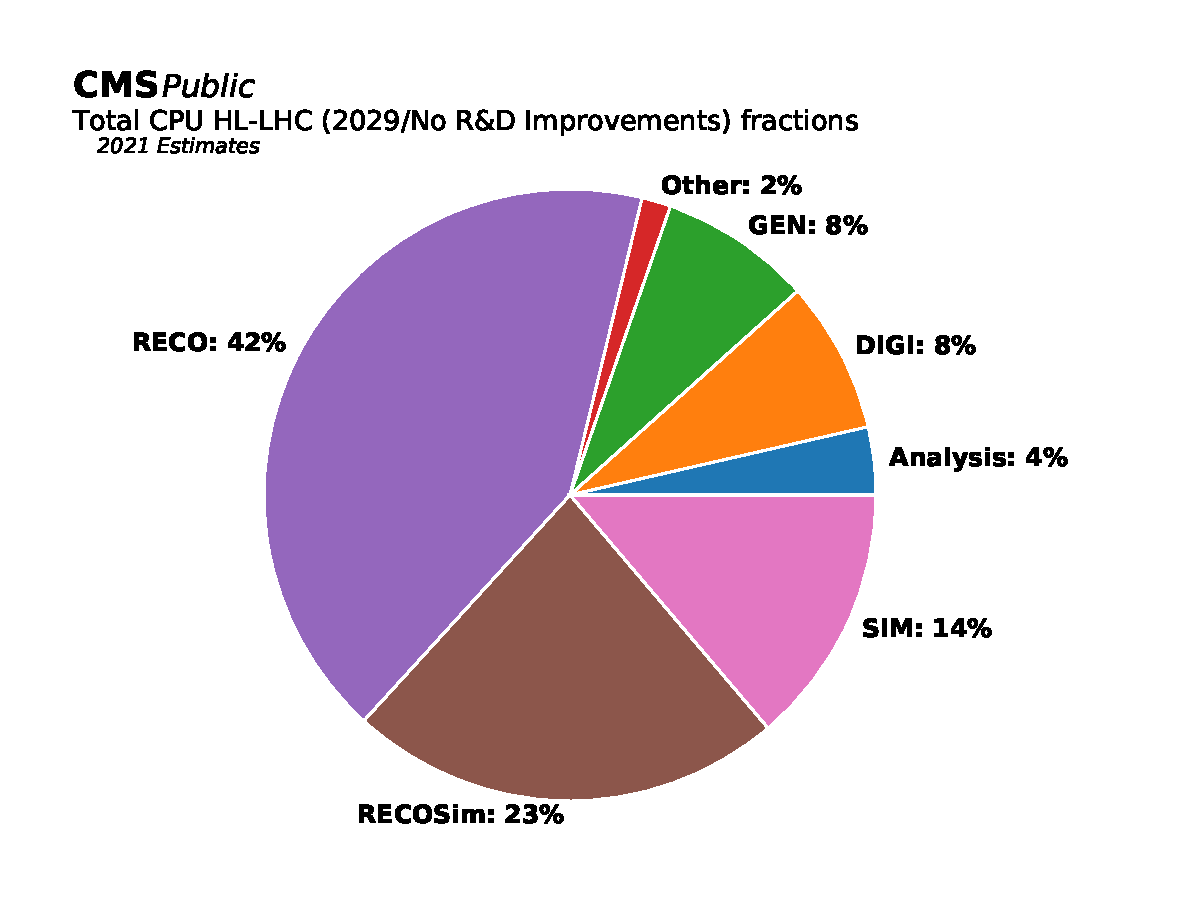
\includegraphics[width=.65\columnwidth]{gfx/ch2/cpu_pie_cms2021.pdf}} 
    \caption[Computing estimates]{The total CPU utilization projections (a) and the approximate breakdown of CPU time into primary processing and analysis activities (b) for the CMS experiment.}\label{fig:cpuusage}
\end{figure}

The plots show estimates from 2021 made for the CMS contribution to the LHCC November review of HL-LHC computing and common software, which supersede previous results from CMS. Coherently with the CMS Phase-2 Upgrade HLT TDR, an integrated luminosity of 270 fb$^{-1}$ per year at 140 pileup events (5 KHz high level trigger rate) and a 1.2 million seconds heavy-ions run is considered during Run 4. For what concerns Run 5, an integrated luminosity of 350 fb$^{-1}$ per year at 200 pileup events (7.5 KHz high level trigger rate) is considered during Run 5. Two scenarios are considered: the first one is a baseline, which does not include any improvement due to ongoing R\&D activity, and the second one incorporates the most probable outcome of the ongoing R\&D activities. The blue curves (and points) show the annual projected needs, summed across Tier-0, Tier-1 and Tier-2 resource needs in each of these scenarios. The gray band shows the projected resource availability for an example scenario that extrapolates the 2018 CMS pledged resources using an annual increase in available resources of between 10$\%$ and 20$\%$. Results are derived from a bottoms-up model of CMS offline processing activities, including prompt reconstruction, Monte Carlo simulation, data re-reconstruction and all phases of analysis activities. 

We also show the approximate breakdown of CPU time into primary processing and analysis activities during a typical HL-LHC year. The plot corresponds to a snapshot of the year 2029. The baseline scenario is considered, i.e. projected effects from on-going R\&D that will reduce the computing resources needed by CMS are not considered.

The presented figures make it clear that:

\begin{outline}
    \1 Both the future and the present CPU (as well as Disk) utilization are completely dominated by the event simulation tasks, which leaves out only about 6$\%$ of resources for other necessities;
    \1 Without improvements from the R\&D sector we risk not being able to meet the future necessities of the collaboration.
\end{outline}


\subsection{Fast simulation}

Clearly, the possibility of performing fast simulations would be a major improvement over the current simulation pipeline, and there are already many different studies and approaches for doing so.

\paragraph{Top-down approach}

In this type of approach, we search for the slowest part of our process and find ways of making it as fast as possible with specific parametric shortcuts. The CMS Collaboration has actually a dedicated approach called CMS \emph{FastSim}, see \cite{https://doi.org/10.48550/arxiv.1701.03850}. 

While FullSim uses the exact detector geometry, tracks particles in small steps, and uses
detailed models for material interactions, FastSim uses a simplified geometry with infinitely thin material layers and simple analytical material interaction models that are parametrized
and tuned to agree with FullSim. For the digitization step, both FullSim and FastSim do a detailed
emulation of detector electronics and trigger, with small exceptions in FastSim. In the reconstruction step, FullSim employs the standard event reconstruction used for reconstructing the real CMS
data. FastSim uses standard reconstruction for calorimetry and muon systems, but a simplified
reconstruction for tracking, based on smearing and truth information, in order to reduce CPU time.

Performance of FastSim is validated regularly within the official CMS software release val-
idation framework; overall, distributions in FastSim agree with FullSim within $\approx 10\%$.

\paragraph{Bottom-up approach}

The bottom-up approach means that we try to skip detector simulation and digitization all together and go directly to the final objects that we would have reconstructed (electrons, muons, jets, missing transverse momentum, $\dots$). A popular framework is the one of \texttt{DELPHES} fast-simulation, see \cite{de_Favereau_2014}.

It takes as input the most common event generator output and performs a fast and realistic simulation of
a general purpose collider detector. To do so, long-lived particles emerging from the hard
scattering are propagated to the calorimeters within a uniform magnetic field parallel to
the beam direction. The particle energies are computed by smearing the initial long-lived
visible particles momenta according to the detector resolution. As a result, jets, missing
energy, isolated electrons, muons and photons, and taus can be reconstructed. It is oviously not meant to
be used for advanced detector studies, for which more accurate tools are needed, but it can nonetheless perform quickly realistic physics studies without in-depth knowledge of the technicalities.


\begin{table}
\begin{adjustbox}{width={\textwidth},totalheight={\textheight},keepaspectratio}%
    \begin{tabular}{lll} \toprule
        \tableheadline{Simulation framework} & \tableheadline{key aspects} & \tableheadline{speed} \\ \midrule
        FullSim & \tabitem detailed geometry; &  $\mathcal{O}(40$ s) for a t$\overline{\text{t}}$ event \\
        & \tabitem small-step tracking; & \\
        & \tabitem \texttt{Geant4} material modelling; & \\
        & \tabitem  detailed digitization; & \\
        & \tabitem full reconstruction & \\
        \midrule
        FastSim & \tabitem simplified geometry; &  $\mathcal{O}(5$ s) for a t$\overline{\text{t}}$ event \\
        & \tabitem thin material layers; & \\
        & \tabitem simple analytical material modelling; & \\
        & \tabitem  detailed digitization; & \\
        & \tabitem full reconstruction with exceptions & \\
        %postulant quo & westeuropee & sanctificatec \\
        \midrule
        Delphes & \tabitem simple tracking system; &  $\mathcal{O}(0.01$ s) for a t$\overline{\text{t}}$ event \\
        & \tabitem smearing & \\
        %autem vulputate ex & parola & romanic \\
        %usu mucius iisque & studio & sanctificatef \\
        \bottomrule
    \end{tabular}
    \end{adjustbox}
    \caption[Simulation frameworks]{An at-glance comparison between the various simulation frameworks employed at the CMS experiment.}
    \label{tab:simfram}
\end{table}

As Table \ref{tab:simfram} shows, the various fast simulation approaches allow us to obtain significant speedups. However, while CMS FastSim accuracy is constantly being improved, its speed is still somewhat lacking; while \texttt{DELPHES} achieves a marked speedup but sacrifices the realistic detector simulation.

\section{The NanoAOD format}




%*****************************************
%*****************************************
%*****************************************
%*****************************************
%*****************************************
